%=========================Preamble====================================%
\documentclass[12pt] {article}
\usepackage{times}
\usepackage[margin=1in,bottom=1in,top=0.2in]{geometry}

\usepackage{graphicx}
\usepackage{subfig}




%=========================Doc====================================%
\begin{document}
\title{ECE 289A - An Introduction to Reinforcement Learning HW\#1}

\author{Ahmed H. Mahmoud}
\date{October, 10th 2017} 
\maketitle


Figure \ref{fig:fig} shows the regenerated plot from Figure 2.4 in \cite{sutton2011reinforcement}. The figure shows the comparison between \emph{upper confidence bound} (UCB) and \emph{$\epsilon$-greedy} method (with $\epsilon$ =0.1) on $K$-armed bandit problem with $K=10$. The plot was generated by averaging the result of 2000 randomly generated $K$-armed bandits over 1000 steps.  
\begin{figure}[!tbh]
\centering        
   \subfloat {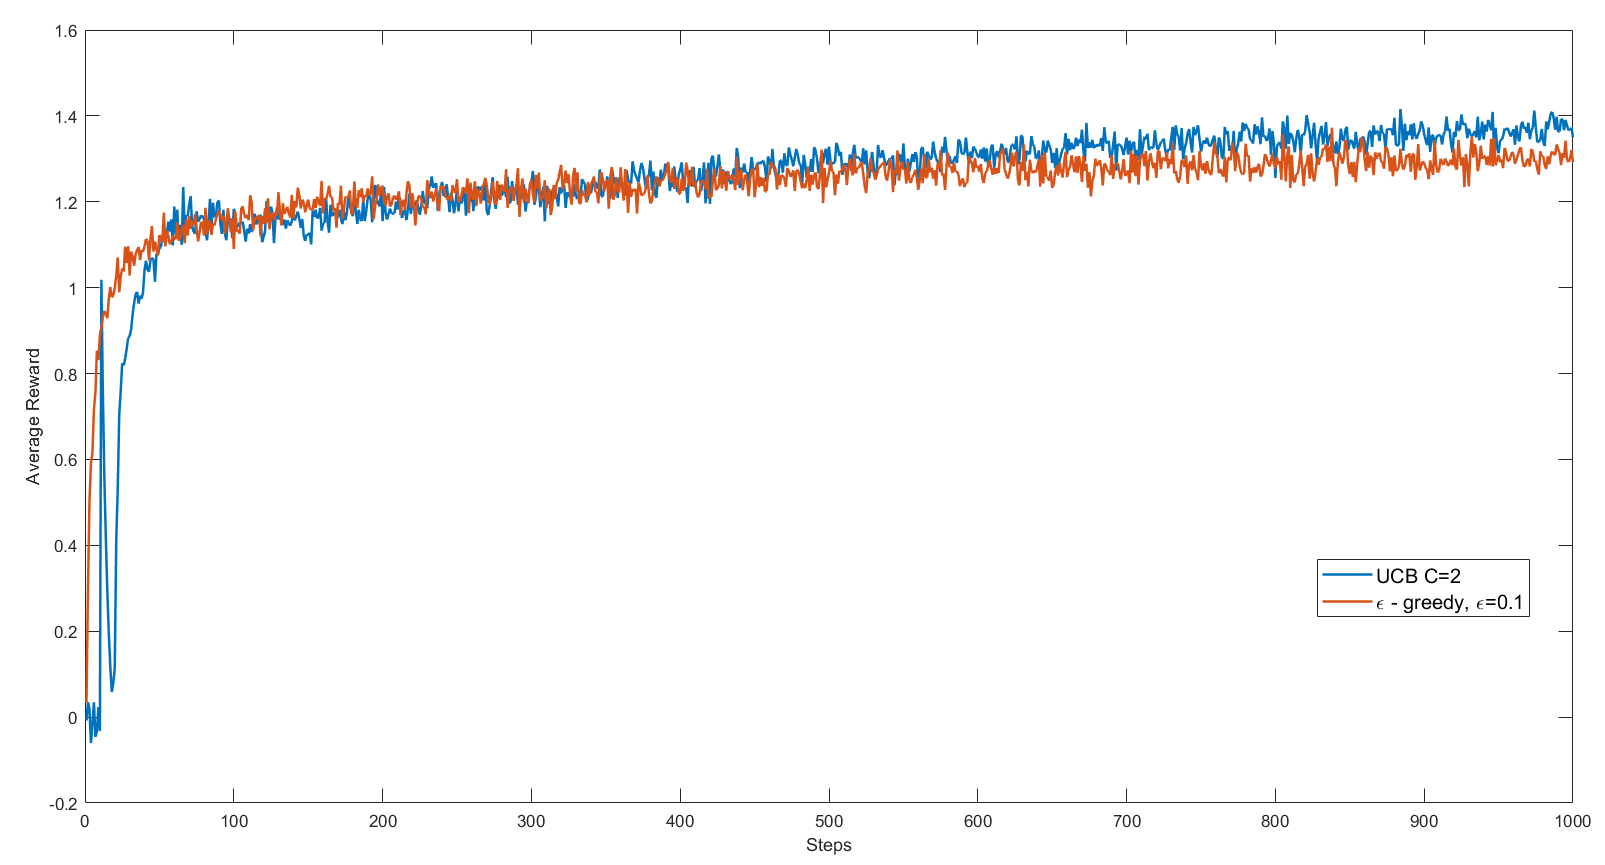
\includegraphics[width=0.65\textwidth]{fig2_4.png}}     
   \caption{ }
   \label{fig:fig}
\end{figure}
We notice that there is a spike on the 11th step on the UCB curve. Since the selection of the next action is based on the following equation 
$$
A_{t} = argmax(Q_{t} (a) + c \sqrt{ \frac{log(t)}{N_{t}(a)}})
$$ 
where $A_{t}$ is the action at time $t$, $Q_{t}(a)$ is the estimate of action $a$ at time $t$, $c$ is the UCB parameter that controls the degree of exploration, and $N_{t}(a)$ is the number of times action $a$ has been taken up to time $t$. At the beginning, all action have $N_{t}(a)=0, \forall a \in K$. Thus, the second term ($c \sqrt{ \frac{log(t)}{N_{t}(a)}}$) is maximum and the action that has not been chosen yet will have a maximum value and will be selected (with random tie breaker). This is will last for first $K$ steps ($K=10$) which guarantees that all actions will be explored first. On the 11th step, all actions will have same value for the second term and only the best action will have a maximum estimate and thus it will be chosen which explains the spike at the 11th step. 




\bibliography{mybib}
\bibliographystyle{plain}


\end{document}
